\documentclass[12pt,parskip=full]{article}
\usepackage{lmodern}
\usepackage{amsmath}
\usepackage[left=1.0in,right=1.0in,top=1.0in,bottom=1.0in]{geometry}
\geometry{letterpaper}
\usepackage{graphicx}
\usepackage{caption}
\usepackage{subcaption}
\usepackage{longtable}
\usepackage{float}
\usepackage{wrapfig}
\usepackage{soul}
\usepackage{textcomp}
\usepackage{marvosym}
\usepackage{wasysym}
\usepackage{latexsym}
\usepackage{amssymb}
\usepackage{apacite}
\usepackage{tabu}
\usepackage[svgnames]{xcolor}
\usepackage{tikz}
\usepackage[linktoc=all]{hyperref}
\usepackage{cleveref}
\usepackage{listings}
\usepackage{setspace}
\usepackage{parskip}
\usepackage{array}
\usepackage{apacite}
\usepackage{natbib}
\usepackage{multicol}
\usepackage{subcaption}
\usetikzlibrary{arrows}

\pgfdeclarelayer{edgelayer}
\pgfdeclarelayer{nodelayer}
\pgfsetlayers{edgelayer,nodelayer,main}

\tikzstyle{none}=[inner sep=0pt]
\tikzstyle{waypt}=[circle,fill=Black,draw=Black,scale=0.4]
\tikzstyle{Helobody}=[circle,fill=White,draw=Black,scale=4.0]
\tikzstyle{Tailrotor}=[circle,fill=White,draw=Black,scale=1.0]
\tikzstyle{ForceVector}=[->,draw=Indigo,fill=Indigo]
\tikzstyle{Coordinate}=[->,draw=Red,fill=Red,fill opacity=1.0]
\tikzstyle{angle}=[->]
\tikzstyle{MeasureMark}=[|-|]
\newlength{\imagewidth}
\newlength{\imagescale}

\setlength{\parskip}{11pt}
%\setlength{\parindent}{15pt}
\usepackage{bookmark}
\makeatletter
\renewcommand\@seccntformat[1]{}
\makeatother

\lstset
{
    language=Matlab,
    keywords={break,case,catch,continue,else,elseif,end,for,function,
        global,if,otherwise,persistent,return,switch,try,while},
    basicstyle=\ttfamily,
    keywordstyle=\color{blue},
    commentstyle=\color{ForestGreen},
    stringstyle=\color{purple},
    numbers=left,
    numberstyle=\tiny\color{gray},
    stepnumber=1,
    numbersep=10pt,
    backgroundcolor=\color{white},
    tabsize=4,
    showspaces=false,
    showstringspaces=false
}

\renewcommand{\thesection}{\arabic{section}}

\renewcommand{\thesubsection}{\thesection\alph{subsection}}
\renewcommand{\theequation}{\thesubsection\arabic{equation}}

\numberwithin{subsection}{section}

\begin{document}
	\vspace{-2ex}
	\title{Report 5: No More Gradients\vspace{-3.5ex}}
	\author{Rob Rau\vspace{-4ex}}
	\date{\today\vspace{-4ex}}
	\maketitle
	
	\section{Discontinuous Drag}
		The optimal point for the discontinuous drag function was found at an aspect ratio of 17.26556792952655428053
		and a reference area of 12.47437282908214406518 $m^2$, with drag equal to 191.59805549860368500958 N. This was
		found using my particle swarm optimizer using 40 particles. Below, \cref{Fig:psoPoints} shows the paths that 5
		of the 40 particles took to reach the minimum as well as the path the BFGS algorithm took.
		\begin{figure}[!ht]
			\centering
				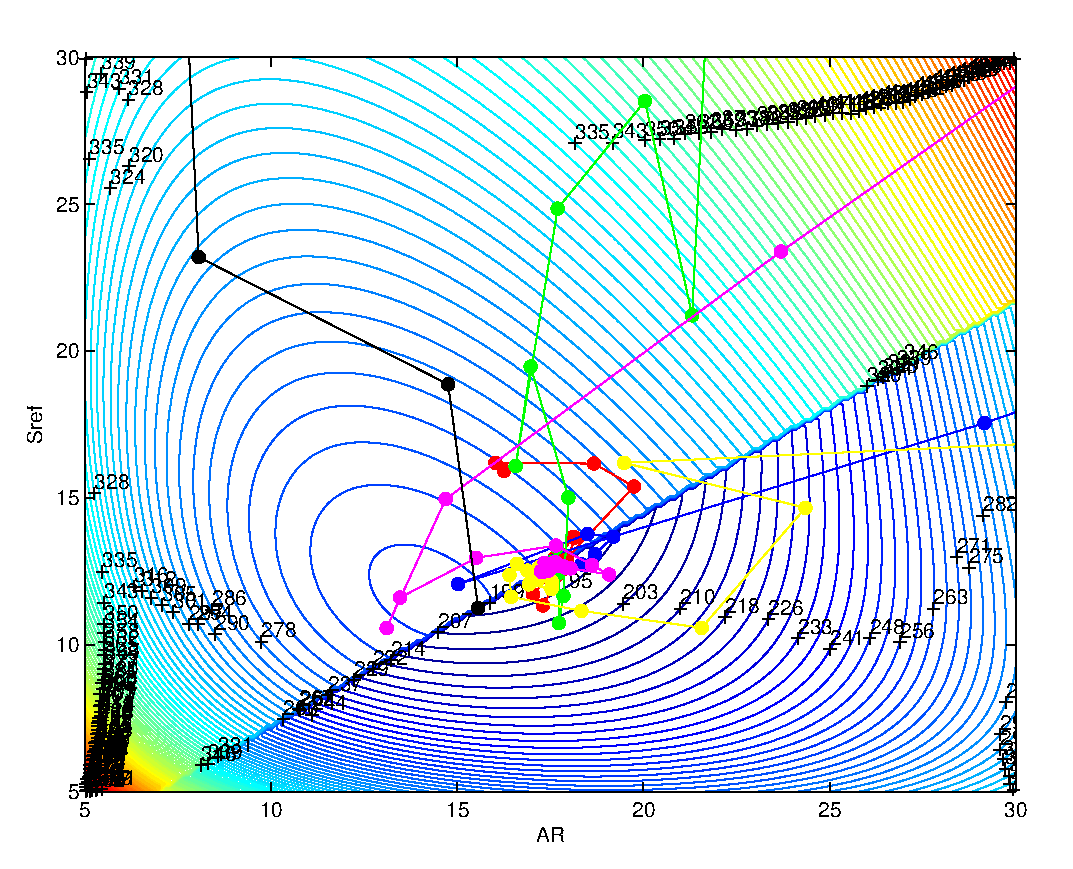
\includegraphics[scale=0.9]{ParticleSwarmDragPoints2.eps}
			\caption{5 particles converging on the minimum. The black path is for BFGS.\label{Fig:psoPoints}}
		\end{figure}
		
		To make the BFGS algorithm work with this type of discontinuous problem, only a minor modification needed to
		be made. Normally the stop conditions for BFGS look at both the convergence of the function value and the
		normalized value of the gradient. This becomes a problem with discontinuous problems as the gradient at the
		minimum point is not necessarily zero. With the default stopping conditions for BFGS, if it was started 
		on one side of the discontinuity it would converge to the drag value of the fully turbulent problem. If 
		started on the other side, it would get confused an stall out. I changed the stopping conditions so it only
		took into account the convergence rate, and would stop when it was below a certain tolerance.
		
		This didn't fully fix the problem, but it was a significant improvement. Now depending on where BFGS was
		started it would still converge to slightly different values. For example, with a starting point of
		$AR = 35$ and $S_{ref} = 10$, BFGS converged to a drag value of 191.90162587272661198767 N. With a starting
		point of $AR = 15$ and $S_{ref} = 40$, BFGS converged to 194.05158969490773301914 N. I did not have time to
		further explore this phenomenon.
		
		The particle swarm optimizer would consistently converge within $0.005\%$ of the same value every time.
		However, to achieve this consistency, a lot of tuning was done to the coefficients. For this problem,
		the coefficients I found to work the best were, $w = 0.5$, $c_1 = 0.6$, $c_2 = 0.9$, and $\Delta t = 0.9$.
		However, when optimizing other problems, like the Rosenbrock function (especially at higher dimensions), 
		I found that these were not the best coefficients.
		
	\section{Performance \& Convergence}
		Finding the proper stopping conditions for the PSO was a source of difficulty for me. The problem with using
		the standard convergence rate of
		\begin{equation}
			\gamma = \frac{ || x_{k+1} - x_k || }{1 + || x_k ||} + \frac{ | f(x_{k+1}) - f(x_k) | }{1 + | f(x_k) | }
		\end{equation}
		is that successive steps may still have the same global optimum if no new one was found. I tried a few
		different methods of measuring the convergence, but the one I found to work best was this:
		\begin{equation}
			\gamma = \frac{ || x^g - \bar x^l || }{1 + || \bar x^l ||} + \frac{ | f(x^g) - f(\bar x^l) | }{1 + | f(\bar x^l) | }
		\end{equation}
		where $x^g$ is the global best optimum so far, and $\bar x^l$ is the average of all particles local optimum.
		I based this on the idea that as the algorithm progresses, the swarm should move closer to the global optimum.
		As it approaches the optimal point, all particles should start converging on the same value. This isn't perfect
		however; if a global optimal point is found that is not the actual optimal there is a chance that that the
		particles converge on the wrong point. I found this to be especially problematic at higher dimensions. This
		problem can be combated by using more particles, but this, of course, uses much more processing power.
		
		Relative to BFGS, the particle swarm algorithm does not perform nearly as well, neither in convergence rate,
		or computational time. This should be intuitively obvious though, as by definition, a particle swarm will
		require many more function evaluations than any gradient based algorithm. Further, in the very early stages of
		the algorithm, there is little guidance of the particles, meaning little progress may be made. A gradient based
		algorithm will have at least an idea of which direction to travel for the very first iteration.
		
		The BFGS algorithm always converged faster. It's shown in \cref{fig:converg} that BFGS always, without a doubt
		converges sooner than PSO. Couple this with the fact that PSO requires many more function evaluations per
		iteration, and PSO starts looking like a bad idea. However, if accurate derivatives are not viable for whatever
		reason, then PSO is probably the best of the worst.
		\begin{figure}[!ht]
			\centering
			\begin{subfigure}[h]{0.45\textwidth}
				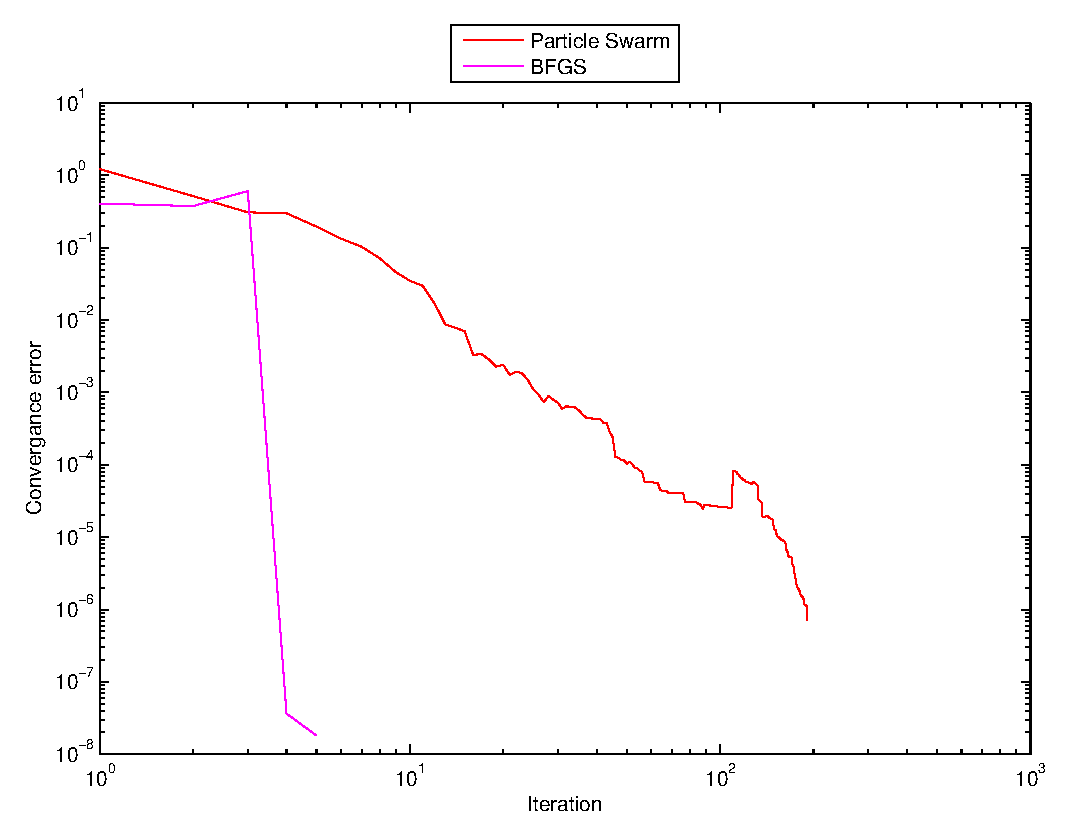
\includegraphics[width=\textwidth]{ParticleSwarmDragError2.eps}
				\subcaption{Drag minimization}
			\end{subfigure}
			\begin{subfigure}[h]{0.45\textwidth}
				\includegraphics[width=\textwidth]{ParticleSwarmRose2DError.eps}
				\subcaption{2 Dimensional Rosenbrock minimization}
			\end{subfigure}
			\begin{subfigure}[h]{0.45\textwidth}
				\includegraphics[width=\textwidth]{ParticleSwarmRose4DError.eps}
				\subcaption{4 Dimensional Rosenbrock minimization}
			\end{subfigure}
			\begin{subfigure}[h]{0.45\textwidth}
				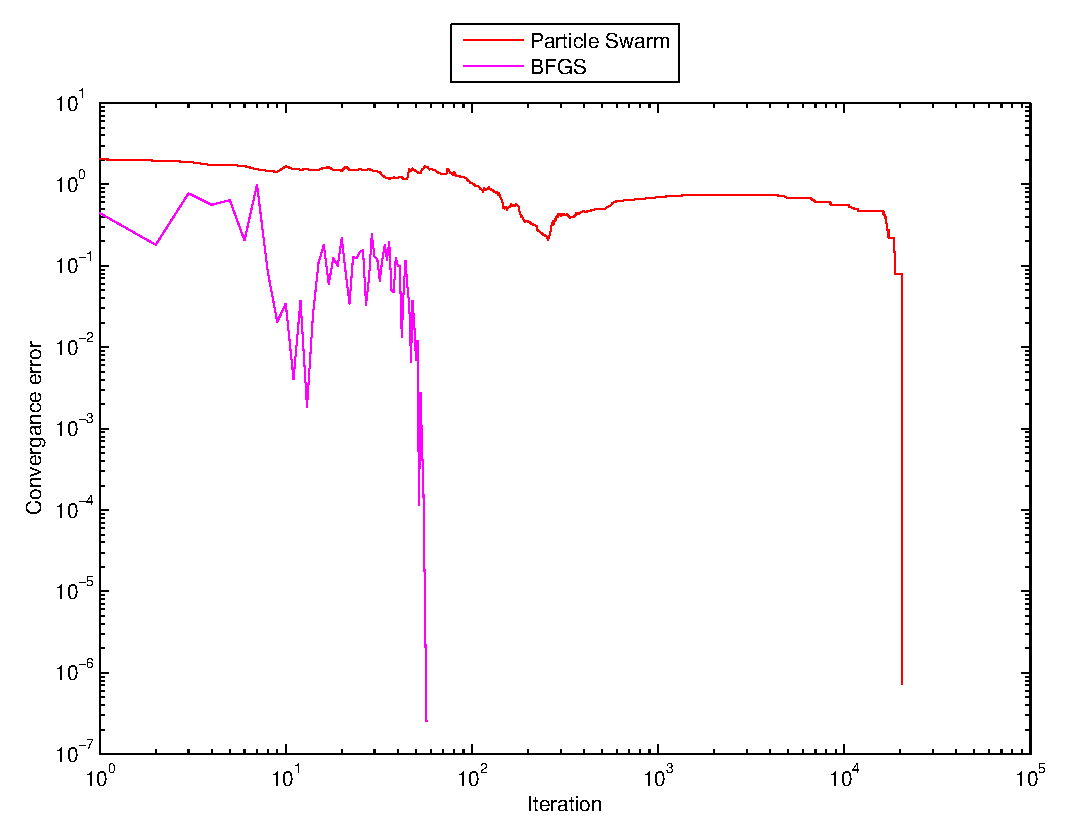
\includegraphics[width=\textwidth]{ParticleSwarmRose8DError.eps}
				\subcaption{8 Dimensional Rosenbrock minimization}
			\end{subfigure}
			\caption{Comparison of convergence rates between BFGS and PSO.\label{fig:converg}}
		\end{figure}
		
	\section{Rosenbrock}

		Increasing the dimensionality of the problem proved somewhat problematic for PSO. The coefficients I found that
		worked best for the two dimensional, did not scale up very well. Using those same constants for the eight
		dimensional case, PSO would consistently converge to the wrong solution. After some further tuning, it would
		converge to the correct solution, but the computation cost increased dramatically. This could be further improved
		with more tuning of the constants, but this underlines a major drawback of the algorithm. Each problem set may need
		different constants for PSO to be effective. This isn't always easy to do, and with an expensive computational
		model it can become impractical to tune the constants. Frankly, the constants themselves present an optimization
		problem that could be solved, but I digress.
		
		I decided to look at the solution error as a function of dimensions using the same constants. As shown in
		\cref{fig:dimError}, an exponential trend emerges as the number of dimensions increase. 
				
		\begin{figure}[!ht]
			\centering
				\includegraphics[scale=0.9]{DimensionError.eps}
			\caption{Error as a function of dimensions.\label{fig:dimError}}
		\end{figure}
		This may very be a result of how I determine convergence, but unfortunately I don't have enough to fully explore
		this (something about having to build an airplane).
		
		Measuring computation time can be troublesome as it can vary somewhat significantly between to independent runs
		of the same problem. However, in theory, increased dimensionality would not have an effect on computation time,
		if the same number of particles are used over a fixed number of iterations. The objective function will still
		only be evaluated once for each particle. Of course this does not take into account stopping criteria or the
		coefficients used for the problem, but again, I did not have time to explore this to the extent I wanted.
		
	\section{Conclusions}
		
		The particle swarm optimizer is an effective choice if accurate gradients aren't available, but it has it's problem
		areas. It can be difficult to tune the constants to a specific problem, something that might be necessary to
		get a decent convergence rate, it is not deterministic, it will not produce the same results each time it is
		run, and the choice of good stopping conditions proved difficult. That being said, it handles discontinuities 
		much better than any gradient based solution and implementation wise, it is much simpler to get running.
		Performance wise, it was very slow compared to BFGS. Even if it converged in the same number of iterations it 
		still takes more computation time if there are an appreciable number of particles. At the end of the day, a
		gradient based solution is the way to go when possible.
	
				
\end{document}
